\section{Results and Discussion}\label{sec:result}

\begin{figure*}
    \centering
    \begin{subfigure}[b]{0.495\textwidth}
    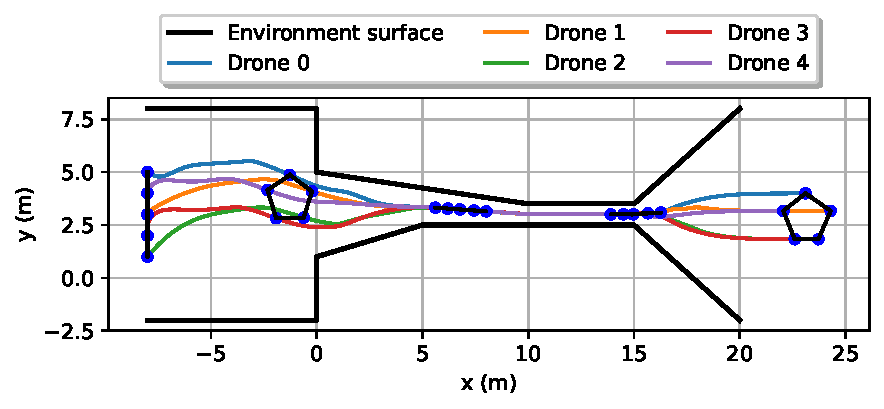
\includegraphics[width=\textwidth]{paper3/images/path_scen1.pdf}
    \caption{Scenario 1 - Motion paths}
    \end{subfigure}
    \begin{subfigure}[b]{0.495\textwidth}
    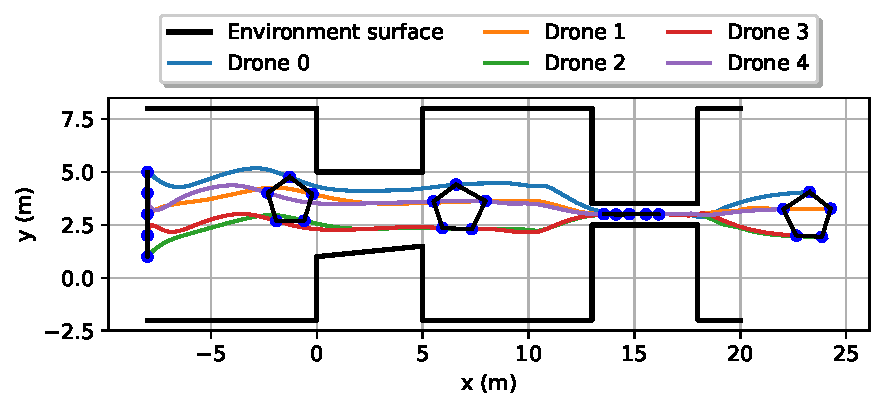
\includegraphics[width=\textwidth]{paper3/images/path_scen2.pdf}
    \caption{Scenario 2 - Motion paths}
    \end{subfigure}
    \begin{subfigure}[b]{0.495\textwidth}
    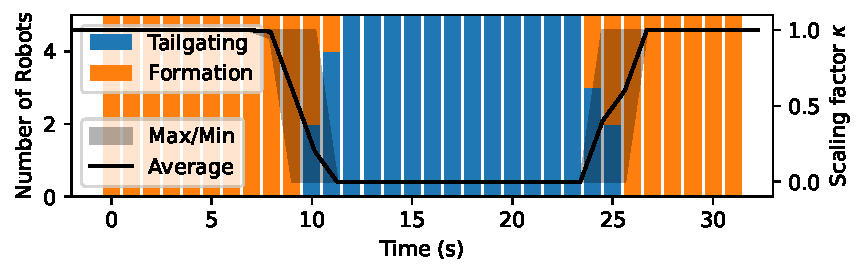
\includegraphics[width=\textwidth]{paper3/images/correlation_scen1.pdf}
    \caption{Scenario 1 - Correlation of number of robots and scaling factor}
    \label{fig:cor1}
    \end{subfigure}
    \begin{subfigure}[b]{0.495\textwidth}
    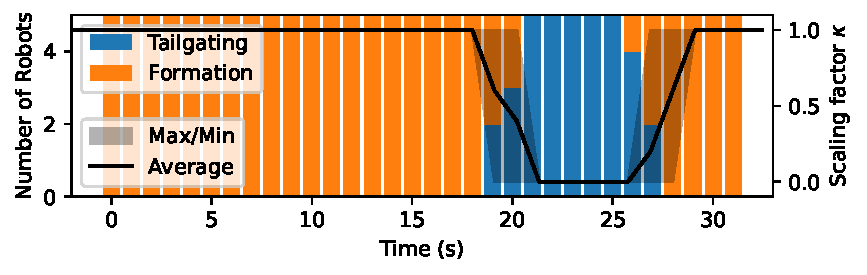
\includegraphics[width=\textwidth]{paper3/images/correlation_scen2.pdf}
    \caption{Scenario 2 - Correlation of number of robots and scaling factor}
    \label{fig:cor2}
    \end{subfigure}
    \caption{The motion path of a pentagon formation in two scenarios using the proposed strategy.}
    \label{fig:path}
\end{figure*}

In this section, our proposed model prediction-based perceptual formation reconfiguration control strategy \textit{(MPPRFC)}, is examined and evaluated through simulation experiments in various cave-like scenarios as depicted in Fig.~\ref{fig:path} and compares with the behavior-based formation reconfiguration control strategy \textit{(BFRC)}, which is reconstructed based on the original model~\cite{736776,Vsrhelyi2018}, and the model prediction-based formation control method \textit{(MPFC)}~\cite{Soria2021,9562281}. For comparison between the different methods, the following performance metrics are used: success rate, mean \textit{order} $\Phi$, mean speed (m/s), mean formation error $\varepsilon$ (m), and acceleration cost $(\sum{\left\Vert u(k)\right\Vert^2}/{N})$ (m$^2$/s$^3$)~\cite{Zhang2021}.

The robot swarm has five homogeneous individuals with size $r=0.2$~m, equipped with a local sensor with a maximum sensing range of $r_s=3$~m. The maximum speed is $\left\Vert v_\text{max}\right\Vert=1.5$~m/s and the maximum control is $\left\Vert u_\text{max}\right\Vert=2.0$~m/s$^2$. In both scenarios, the desired velocity during movement is set to $\bar{v}_\text{ref}=1$~m/s. The desired formation is set as a regular pentagon. Initially, all robots are randomly positioned on one side of the zone. The swarm then navigates through the narrow passages in the zone along the desired direction $u_\text{ref}=[1,0,0]^T$. The mission is considered complete when all the robots have crossed to the opposite side of the region, specifically $p_x\geq22.0$ in all scenarios. The control period of robots is set at $\tau=0.1$~s.

The \textit{order} $\Phi$ metric~\cite{Vicsek1995} is used to measure the heading consensus of robots in formation during movement. The order value is in $\left[0,1\right]$. If robots in the formation have the same direction, the order value is close to 1. It is defined as follows. 

\begin{equation}
    \Phi=\dfrac{1}{N}\left\Vert\sum_{i=1}^N{\dfrac{v_i}{\left\Vert v_i\right\Vert}}\right\Vert
\end{equation}

To demonstrate the effectiveness in maintaining the formation, the \textit{formation error} evaluates the deviation between the actual position $p_i$ and its expected position $p^*_i$ of all robots in the formation to demonstrate the effectiveness of the formation control strategy~\cite{6798711}. The closer this error is to zero, the more effective the controller becomes. The formation error $\varepsilon_i$ of robot $i$ can be calculated as follows:
\begin{equation}
    \varepsilon_i = \left\Vert p_i-p^*_i\right\Vert
\end{equation}

\subsection{Results and Comparisons}
\label{subsec:results}

\begin{figure*}[h!]
    \centering
    \begin{subfigure}[b]{0.495\textwidth}
    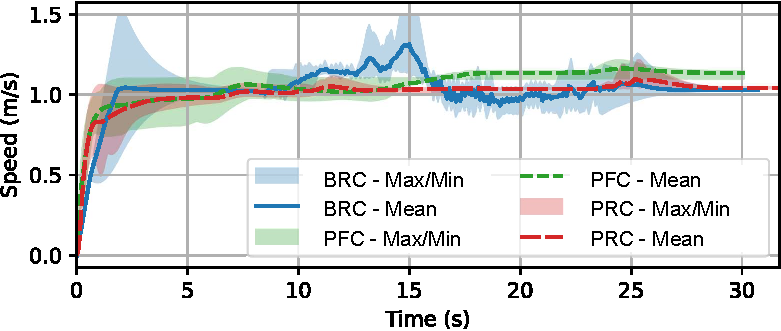
\includegraphics[width=\textwidth]{paper3/images/velocity_scen1.pdf}
    \caption{Scenario 1 - Speed}
    \label{fig:speed1}
    \end{subfigure}
    \begin{subfigure}[b]{0.495\textwidth}
    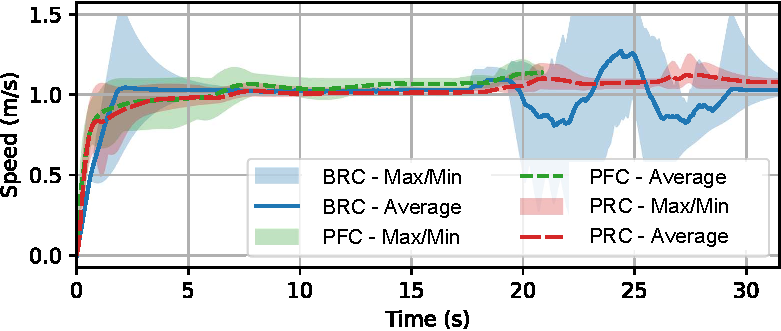
\includegraphics[width=\textwidth]{paper3/images/velocity_scen2.pdf}
    \caption{Scenario 2 - Speed}
    \label{fig:speed2}
    \end{subfigure}
    \begin{subfigure}[b]{0.495\textwidth}
    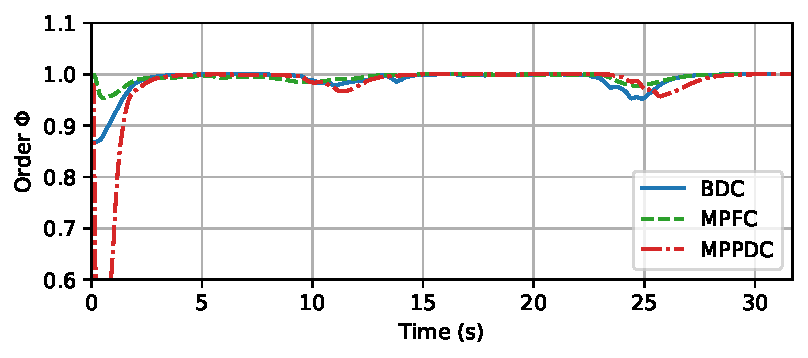
\includegraphics[width=\textwidth]{paper3/images/order_scen1.pdf}
    \caption{Scenario 1 - \textit{Order} $\Phi$}
    \label{fig:order1}
    \end{subfigure}
    \begin{subfigure}[b]{0.495\textwidth}
    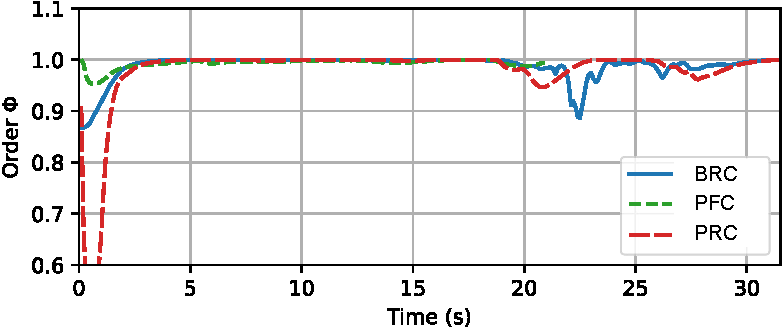
\includegraphics[width=\textwidth]{paper3/images/order_scen2.pdf}
    \caption{Scenario 2 - \textit{Order} $\Phi$}
    \label{fig:order2}
    \end{subfigure}
    \begin{subfigure}[b]{0.495\textwidth}
    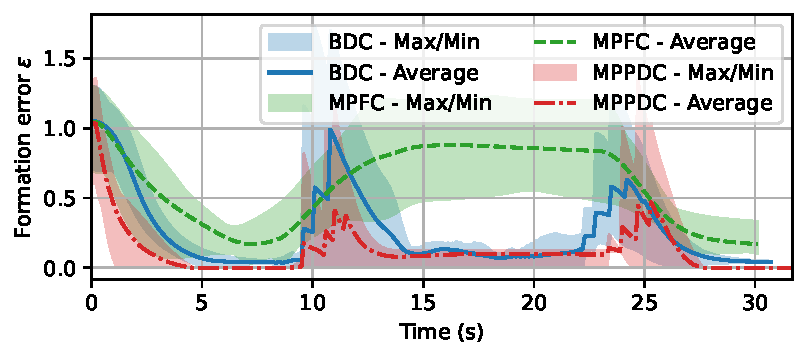
\includegraphics[width=\textwidth]{paper3/images/error_scen1.pdf}
    \caption{Scenario 1 - \textit{Formation error} $\varepsilon$}
    \label{fig:error1}
    \end{subfigure}
    \begin{subfigure}[b]{0.495\textwidth}
    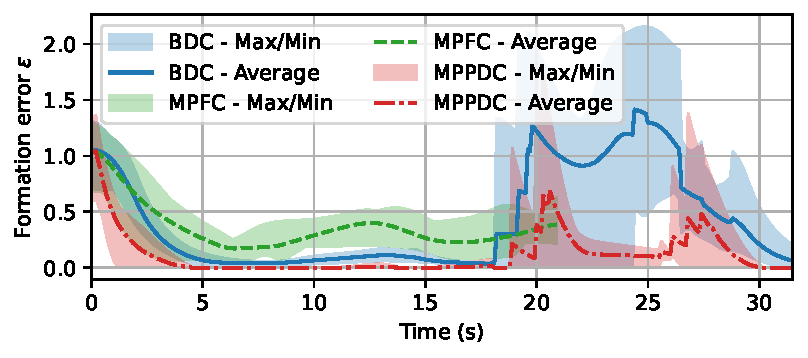
\includegraphics[width=\textwidth]{paper3/images/error_scen2.pdf}
    \caption{Scenario 2 - \textit{Formation error} $\varepsilon$}
    \label{fig:errorr2}
    \end{subfigure}
    \caption{Comparison results of three strategies in two scenarios.}
    \label{fig:comparison}
\end{figure*}

\begin{figure}[h!]
    \centering
    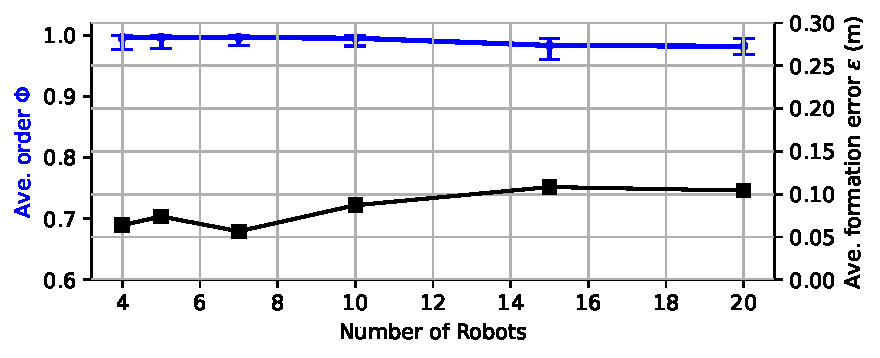
\includegraphics[width=0.6\textwidth]{paper3/images/scalability.pdf}
    \caption{Effect of number of robots on system performance, including \textit{order} $\Phi$ value and formation error $\varepsilon$.}
    \label{fig:scalability}
\end{figure}

According to Fig.~\ref{fig:path}, in both scenarios, the robot's formation successfully passes through the narrow space. At the beginning of the motion, the formation rapidly forms a desired pentagon shape. They then change their shape to safely pass through the tight passages, and then transform back to the desired shape after escaping the passages. Fig.~\ref{fig:cor1}-\ref{fig:cor2} depict the correlation of the number of robots in different modes and scaling factor $\kappa$. It can be seen that our strategy provides distributed decision-making capabilities based on the collected information. In particular, the modes of the robot swarm at a specific time vary depending on the structure of the environment and its neighbors. 

Besides, when the environment is large enough to maintain the original shape, the value of scaling factor $\kappa$ is determined to be 1. When the width of the environment is decreased, the $\kappa$ of each robot is also determined to be smaller than 1 and gradually decreases depending on the width of the passage, adjusting the shape of the formation to shrink. Once the mode is switched to \textit{``Tailgating''}, the $\kappa$ value is determined to be 0. Similarly, when the formation exits the narrow corridor, the width of the environment increases, leading to an increased $\kappa$ value, guiding the formation shape to return to its original shape.

\begin{table*}
\centering
\caption{The comparison between \textit{BFRC}, \textit{MPFC}, and the proposed \textit{MPPRFC}. Each comparison is over 10 simulations of 5 robots in two
different scenarios. The metrics displayed in the table are
the success rate, mean \textit{order}, mean speed, mean formation error, and acceleration cost.}
\label{tbl:analys}
\begin{tabular}{C{1.0cm}C{1.4cm}C{1.8cm}C{1.8cm}C{2.5cm}C{2.3cm}C{2.0cm}}
\hline \hline
Scen.             & Strategy & Success rate  & Mean \textit{order} $\Phi$ & Mean speed (m/s) ($v_\text{ref}=1$~m/s) & Mean formation error $\varepsilon$ (m) & Acceleration cost (m$^2$/s$^3$) \\ \hline
\multirow{3}{*}{1  } & BFRC      & \textbf{10/10} & 0.9890     & 1.0249     & 0.3048               & 69.6589    \\
                     & MPFC     & 8/10  & \textbf{0.9934}     & 1.0639     & 0.6376               & \textbf{23.7442}    \\
                     & MPPRFC    & \textbf{10/10} & 0.9824     & \textbf{0.9863}     & \textbf{0.2423}               & 25.0894    \\ \hline
\multirow{3}{*}{2}   & BFRC      & 6/10  & 0.9883     & \textbf{0.9887}     & 0.6872               & 53.8718    \\
                     & MPFC     & 0/10  & \textbf{0.9953}     & 1.0470      & 0.4593               & \textbf{19.0365}    \\
                     & MPPRFC    & \textbf{9/10}  & 0.9830     & 0.9800       & \textbf{0.3217}               & 21.8559   \\ \hline \hline
\end{tabular}
\end{table*}

To describe the effectiveness of the \textit{MPPRFC} strategy, Fig.~\ref{fig:comparison} illustrates the comparisons of our proposed strategy with other methods including speed profile, \textit{order} metric, and \textit{formation error}. 

Fig.~\ref{fig:speed1}-\ref{fig:speed2} show the speed profiles of three strategies in both scenarios. The proposed strategy has demonstrated the ability to maintain a steady velocity around the desired velocity $v_\text{ref}$. The \textit{BFRC} shows the unstable speed when the formation changes its shape and/or navigates through the narrow passage due to the effect of the environment. Besides, \textit{MPFC} indicates stability in achieving the desired velocity. However, when the robots in formation face a narrow environment, they do not maintain the designed velocity but are slightly larger.

Fig.~\ref{fig:order1}-\ref{fig:order2} present the \textit{order} metric of three strategies. The results show the high consensus of robots in formation, represented by \textit{order} value $\Phi$ approaching~1. Our \textit{MPPRFC} algorithm has demonstrated the ability to navigate formations more stably when encountering changes in narrow environments.

Fig.~\ref{fig:error1}-\ref{fig:errorr2} depict the superiority of the proposed \textit{MPPRFC} algorithm compared to other strategies in terms of formation maintenance. The \textit{BFRC} and \textit{MPPRFC} formation reconfiguration strategies both present well-designed formation maintenance, as evidenced by the formation error converging to zero during movement. It can be seen that the proposed \textit{MPPRFC} controller maintains the designed formation better than \textit{BFRC}. Meanwhile, the configuration error of \textit{MPFC} is very significant, because of the influence of obstacles on the ability to operate.

Table~\ref{tbl:analys} presents a detailed comparison between the \textit{BFRC}, \textit{MPFC}, and the proposed \textit{MPPRFC} strategies. The results demonstrate that the proposed \textit{MPPRFC} strategy outperforms \textit{MPFC} in both scenarios and surpasses \textit{BFRC} in Scenario 2. In Scenario 1, the width-varying tunnel allows the \textit{BFRC} to switch modes and configurations smoothly and efficiently. However, in Scenario 2, where the tunnel's width changes suddenly, the formation struggles to adapt its configuration in time. The proposed \textit{MPPRFC} excels in maintaining the formation due to its minimal formation error, $\varepsilon$.

While the \textit{MPFC} exhibits the best acceleration cost-owing to the absence of transformations between modes-the cost associated with the \textit{MPPRFC} is slightly higher but still shows significant improvement over \textit{BFRC}. Both formation reconfiguration control methods (\textit{MPFC} and \textit{MPPRFC}) demonstrate effective speed maintenance, as they approximately sustain the desired reference speed, $v_\text{ref}$. The mean order in all three strategies is close to 1, reaffirming their efficiency in maintaining the formation.
% Table~\ref{tbl:analys} shows the statistics of three strategies in two different scenarios. It can be seen that, in both experiments, \textit{BFRC} and \textit{MPPRFC} were able to move through different types of narrow passages to reach their target, while \textit{MPFC} was only successful in scenario 1, where the width of the environment changes gradually. In scenario 2, when the width changes suddenly, the \textit{MPFC} cannot pass the narrow passage and collides with obstacles. In both scenarios of \textit{BFRC} and \textit{MPPRFC} strategies, the smallest distance between two robots $d_{ij}$ is always larger than $2r$, i.e. 0.4 m, and the smallest distance between the robot and the obstacles $d_{im}$ is always greater than robot radius $r$, i.e. 0.2 m. This proves that those strategies successfully move through the narrow passages without collisions. 

We further investigate the effect of swarm size on the performance of the proposed strategy by using swarms of 4, 5, 7, 10, 15, and 20~robots. We evaluate the changes in the average \textit{order} value~$\Phi$ and formation error~$\varepsilon$ during the robot swarm's movement, as illustrated in Fig. \ref{fig:scalability}. The results indicate that as the number of robots in the formation increases, the proposed strategy maintains a high level of navigation ability, with the average \textit{order} value remaining close to~1. When considering the influence of the number of robots on the average formation error $\varepsilon$ value, we exclude the formation generation stage and the transition stage. The results show that, as the number of robots in the formation increases, the formation error remains relatively stable, fluctuating around 0.1~m. Additionally, statistics show that the time required to generate a formation from the initial position, $t_1$, and the time needed to switch formations between different modes, $t_2$, both increase as the number of robots in the formation grows. Specifically, for a formation of 4 robots, $t_1 \approx 2.5$~s and $t_2 \approx 2$~s, for a formation of 20~robots, $t_1\approx6.5$~s and $t_2\approx5.2$~s. Overall, the \textit{MPPRFC} algorithm has been shown to be effectively deployable in scalable robot swarms, confirming its robustness and efficiency across various swarm sizes.

\subsection{Software-in-the-loop verification}
\begin{figure*}
    \centering
    \begin{subfigure}[b]{0.56\textwidth}
    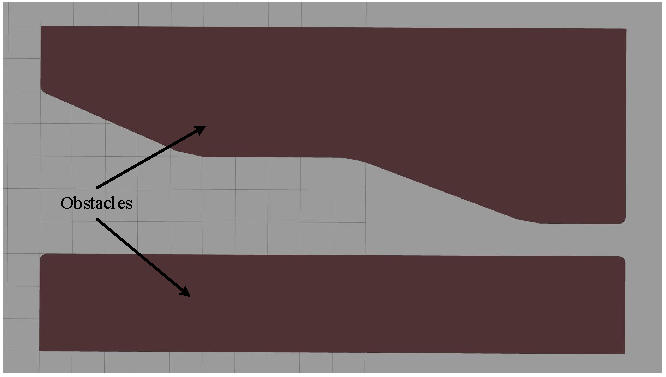
\includegraphics[width=\textwidth]{paper3/images/tunnel.pdf}
    \caption{The cave-like environment}
    \label{fig:gazebo_tunnel}
    \end{subfigure}
    \begin{subfigure}[b]{0.42\textwidth}
    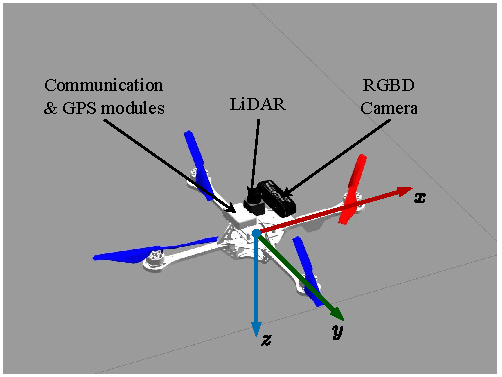
\includegraphics[width=\textwidth]{paper3/images/hummingbird.pdf}
    \caption{The used drone model~\cite{Bui2022,Furrer2016}}
    \label{fig:gazebo_hummingbird}
    \end{subfigure}
    \caption{The SIL set up on Gazebo simulator. The environment consists of two large obstacles forming a cave-like environment. We use 5 Hummingbird drones equipped with perception sensors including LiDAR, RGBD camera, communication and positioning modules.}
    \label{fig:sil}
\end{figure*}
\begin{figure*}
    \centering
    \begin{subfigure}[b]{0.325\textwidth}
    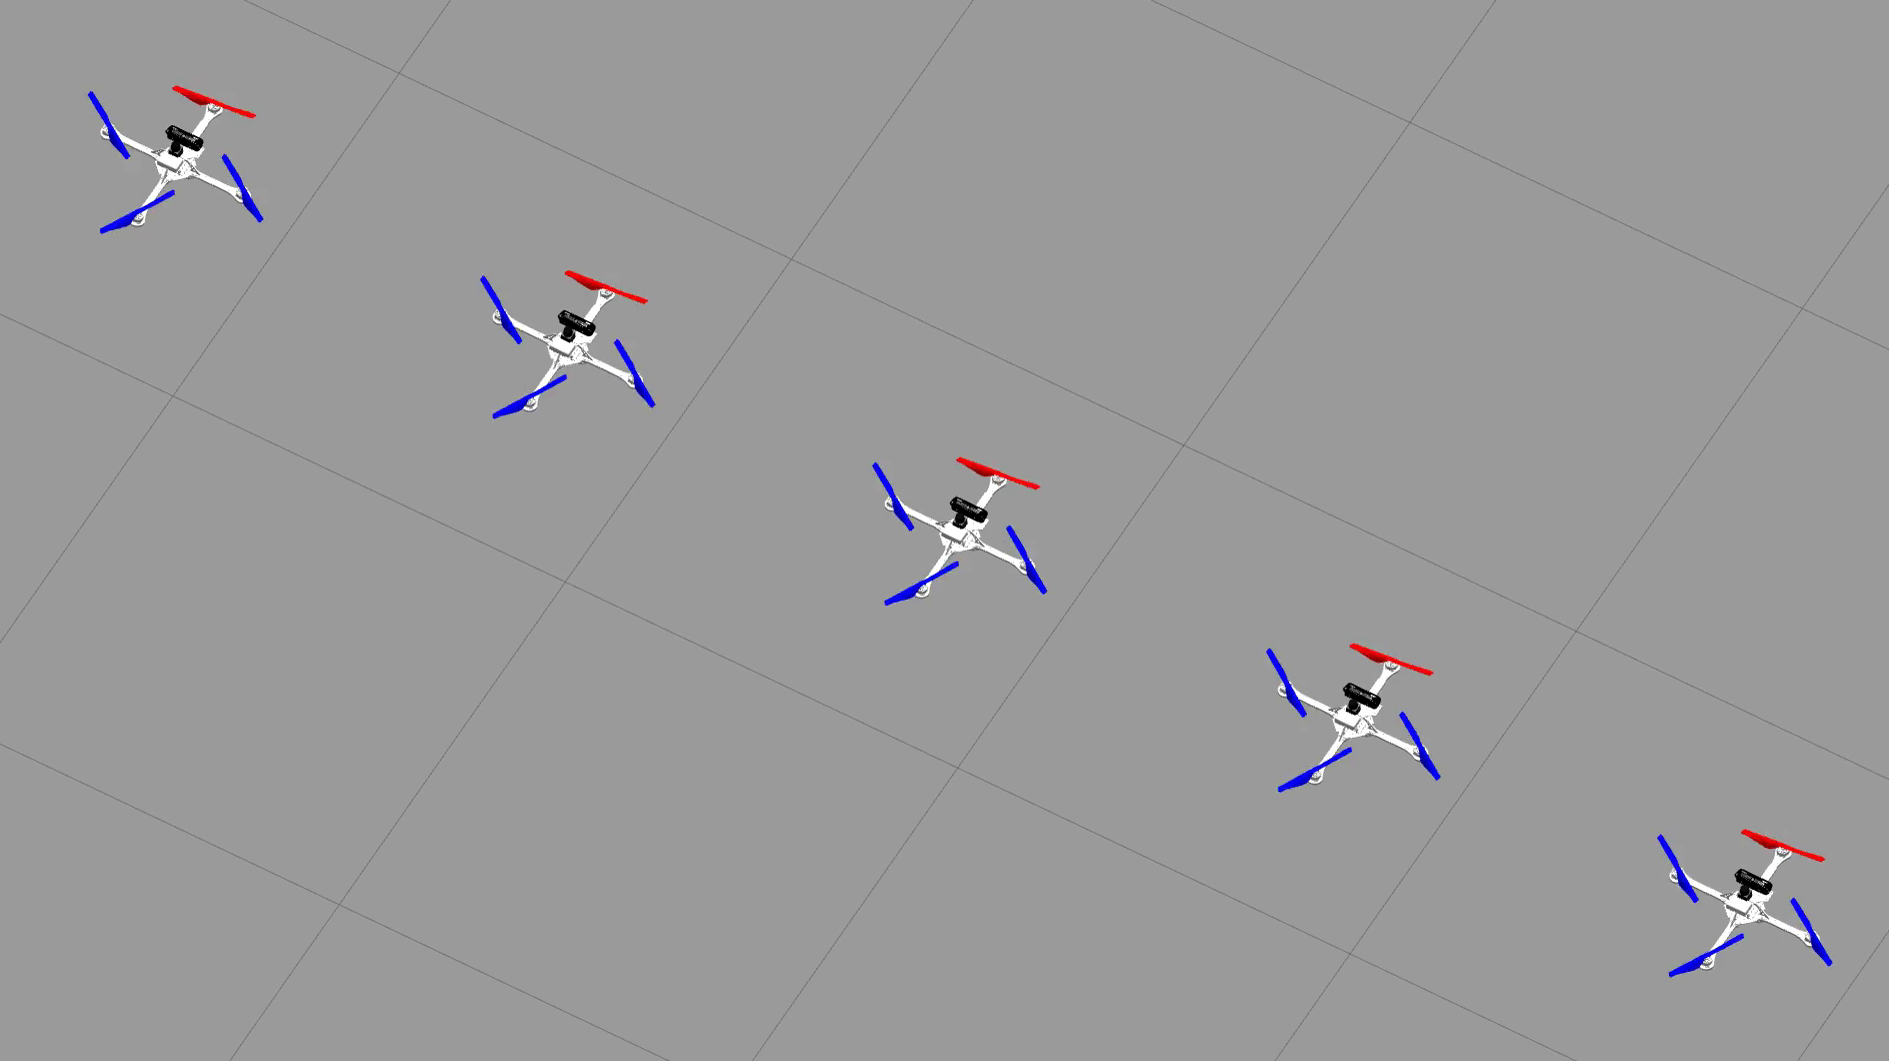
\includegraphics[width=\textwidth]{paper3/images/gazebo_01.png}
    \caption{}
    \end{subfigure}
    \begin{subfigure}[b]{0.325\textwidth}
    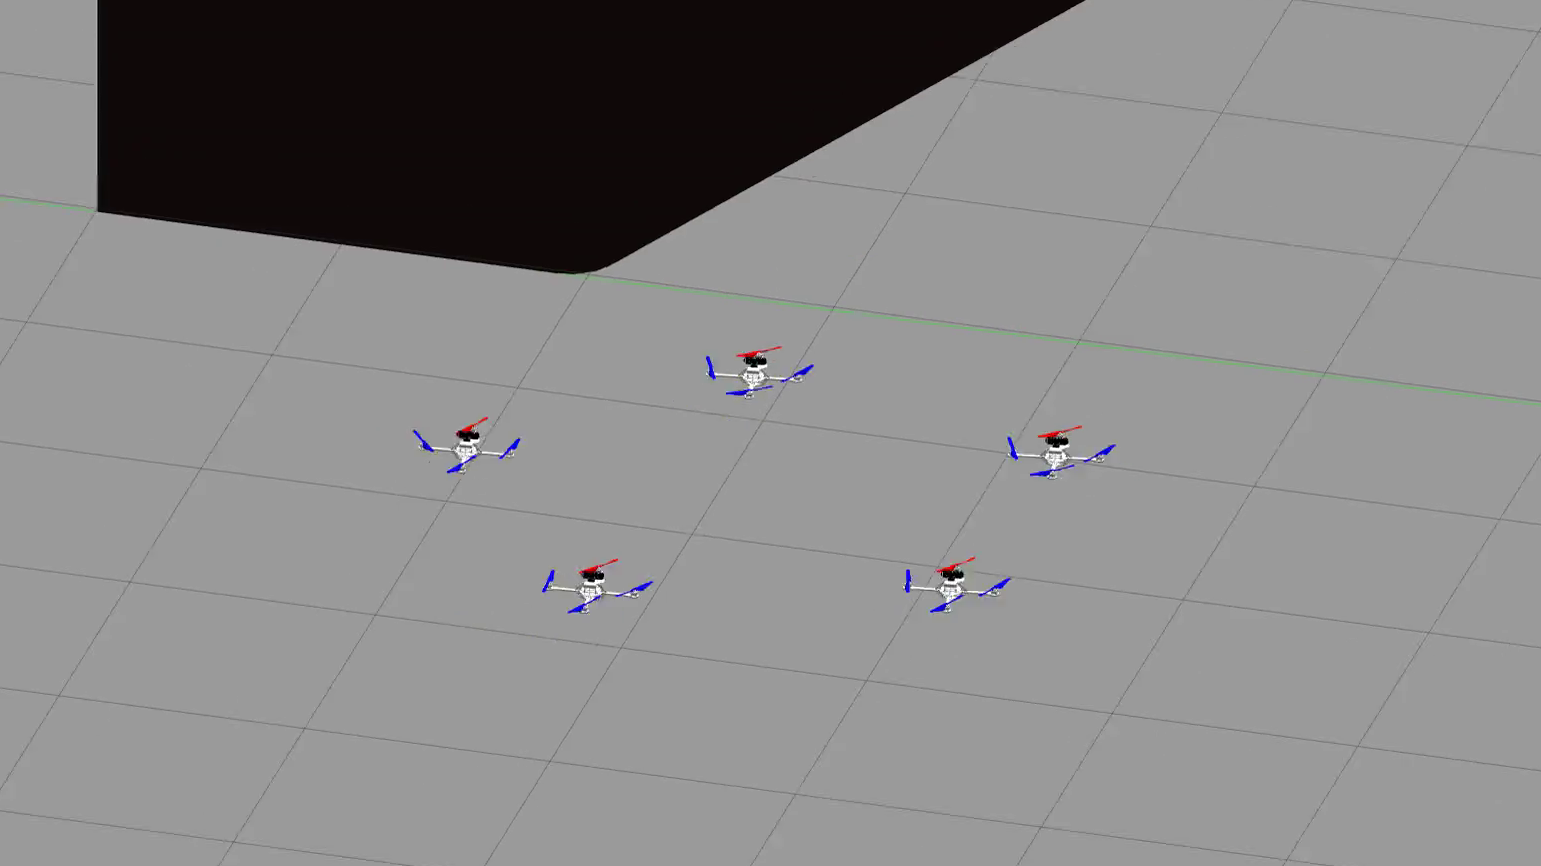
\includegraphics[width=\textwidth]{paper3/images/gazebo_02.png}
    \caption{}
    \end{subfigure}
    \begin{subfigure}[b]{0.325\textwidth}
    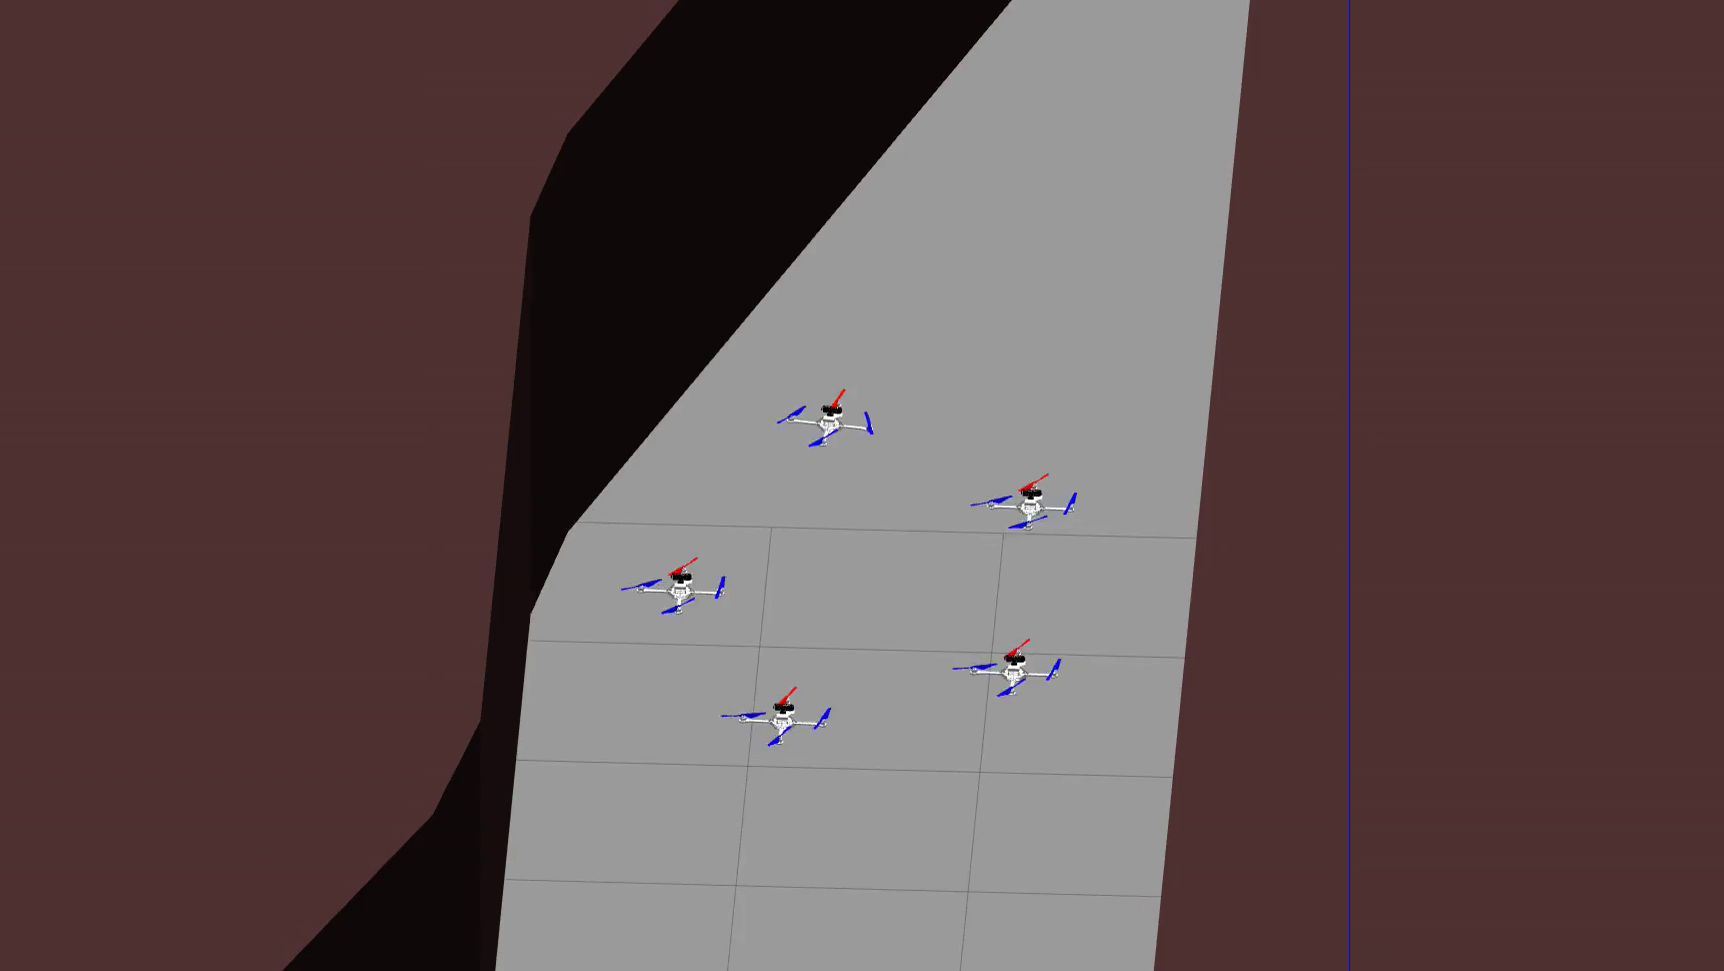
\includegraphics[width=\textwidth]{paper3/images/gazebo_03.png}
    \caption{}
    \end{subfigure}
    \begin{subfigure}[b]{0.325\textwidth}
    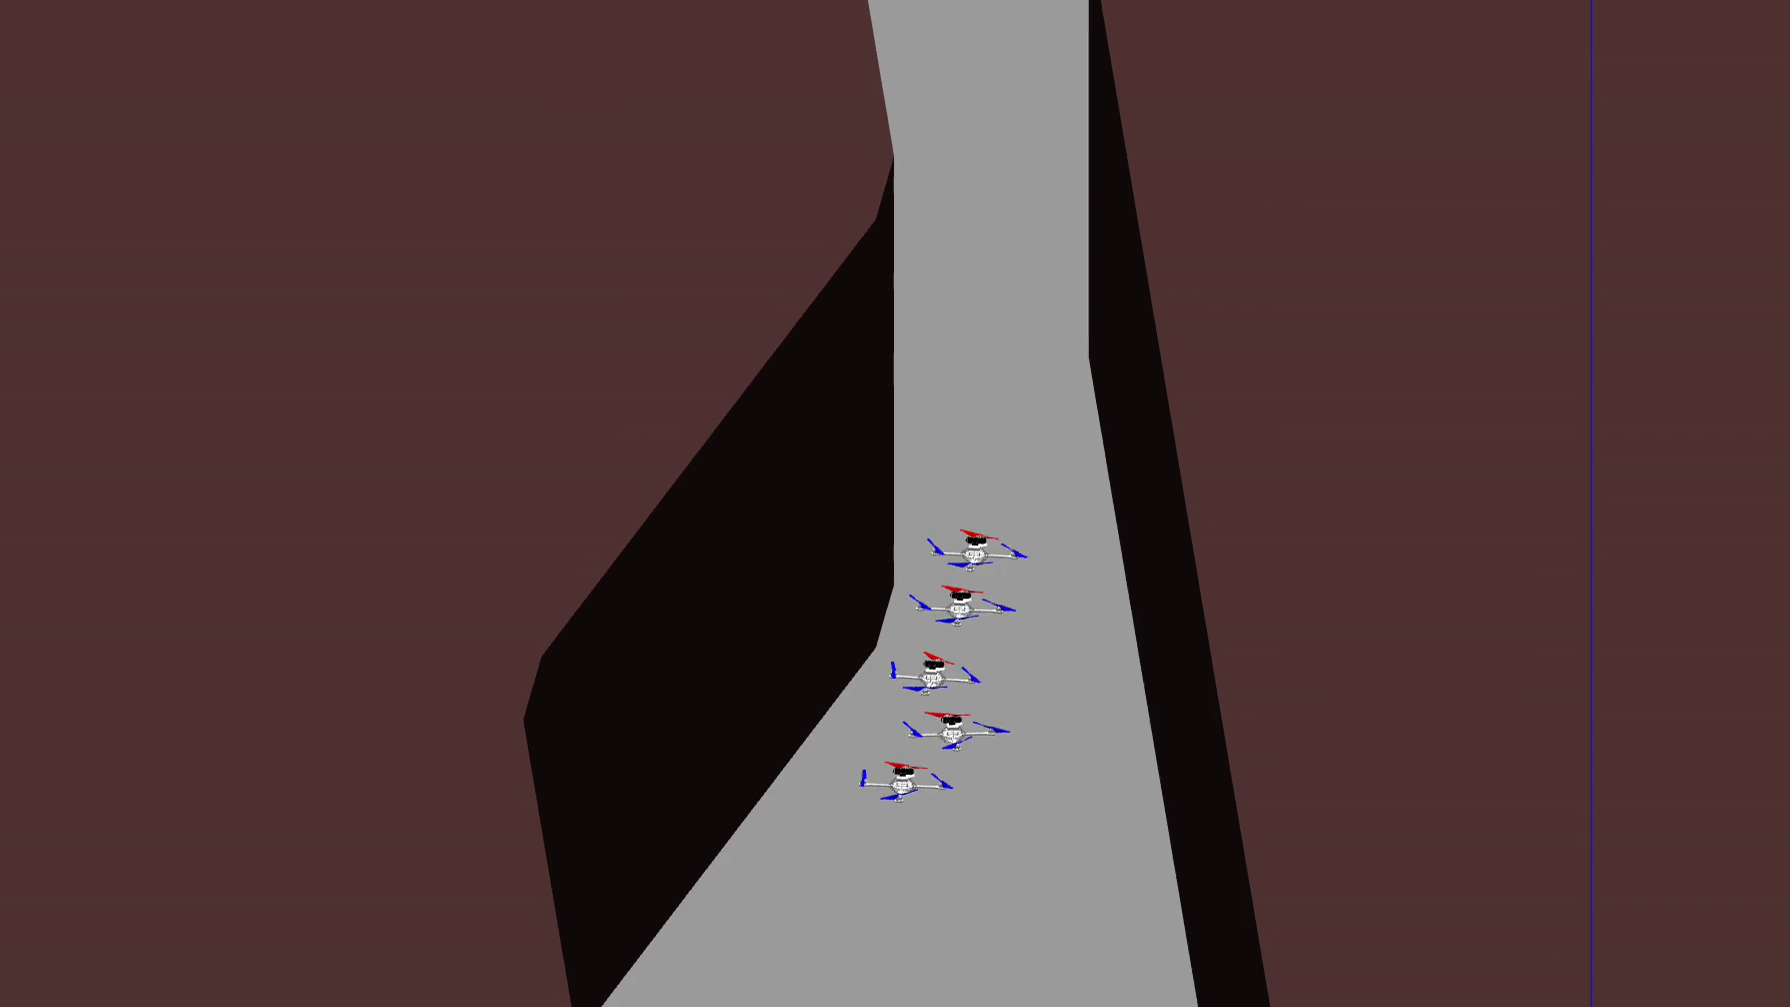
\includegraphics[width=\textwidth]{paper3/images/gazebo_04.png}
    \caption{}
    \end{subfigure}
    \begin{subfigure}[b]{0.325\textwidth}
    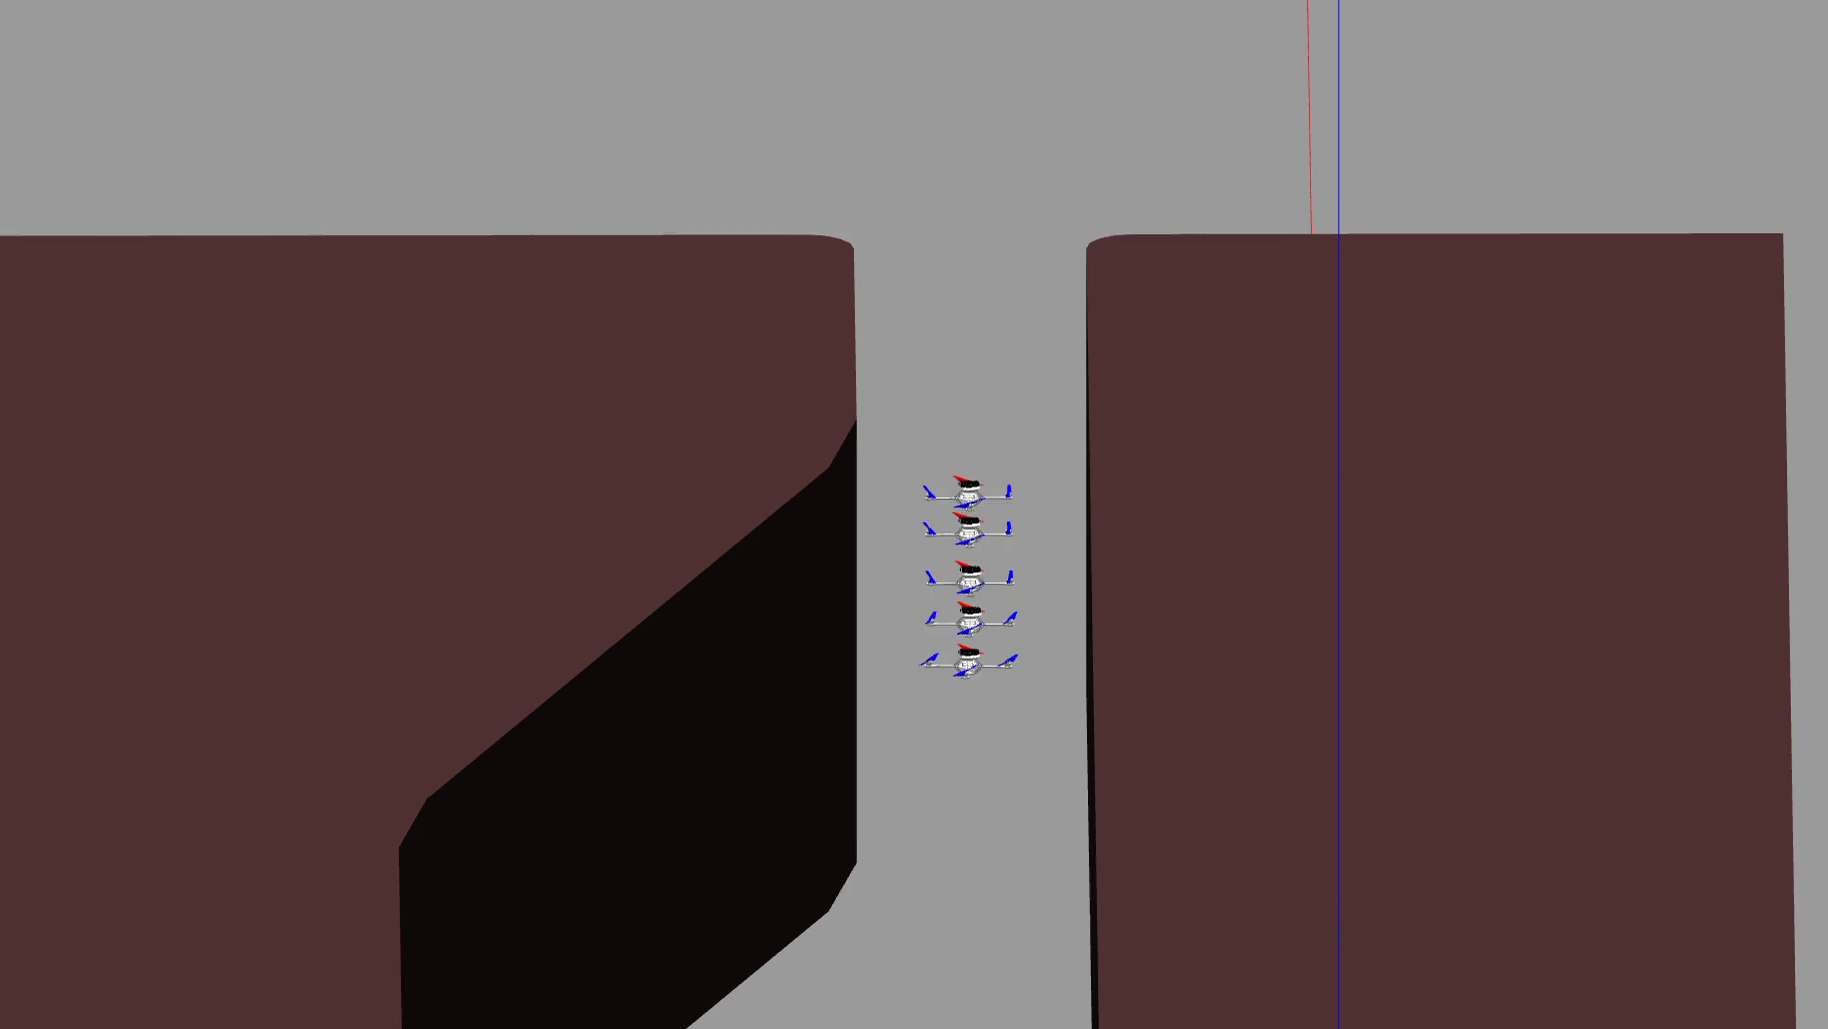
\includegraphics[width=\textwidth]{paper3/images/gazebo_05.png}
    \caption{}
    \end{subfigure}
    \begin{subfigure}[b]{0.325\textwidth}
    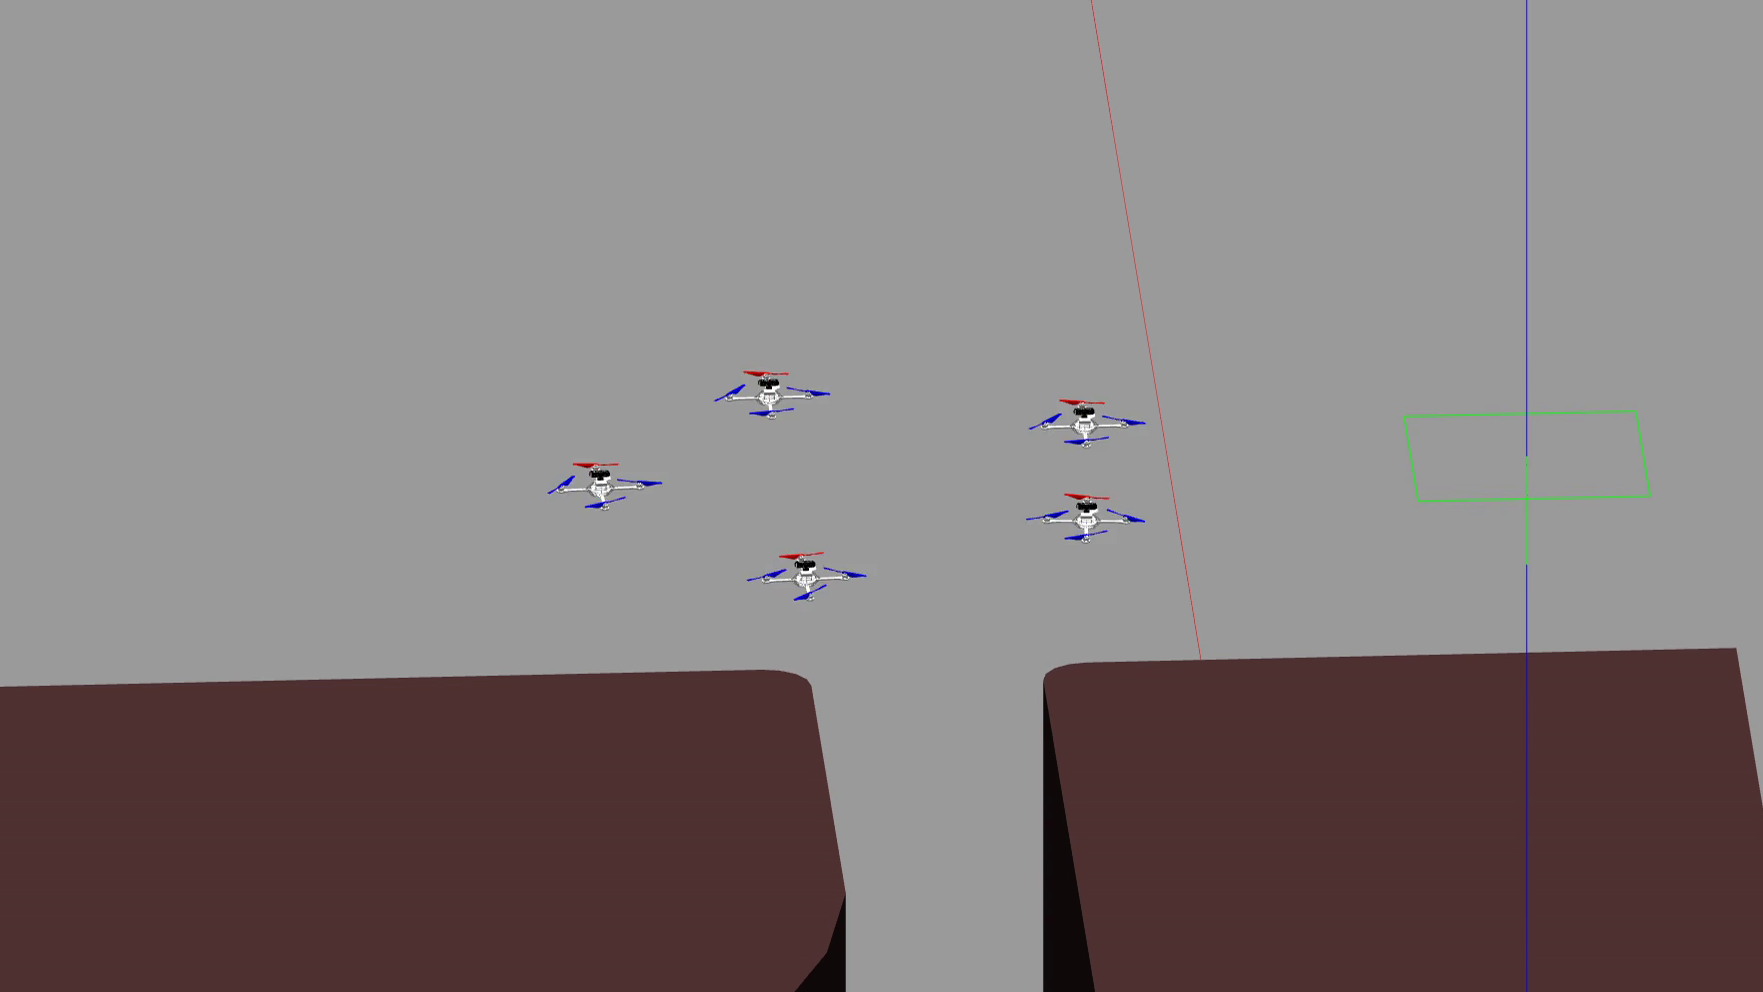
\includegraphics[width=\textwidth]{paper3/images/gazebo_06.png}
    \caption{}
    \end{subfigure}
    \caption{Snapshot of the migration process of a formation using the proposed strategy. At the beginning of the SIL test, drones in a formation hover and start at their initial positions (a). Consequently, they converge to the specified shape (b), i.e. pentagon shape. When they sense that the width of the environment is not enough to maintain their original shape, they deform their shape to adapt to the environment (c). When the formation finds that the environment in the front is too narrow, the formation transforms into a straight line shape (d) and moves safely through the narrow passage (e). Finally, after escaping from the narrow passage, they transform back to their original shape (f) and reach the target.}
    \label{fig:snap}
\end{figure*}

\begin{figure*}
    \centering
    \begin{subfigure}[b]{0.48\textwidth}
    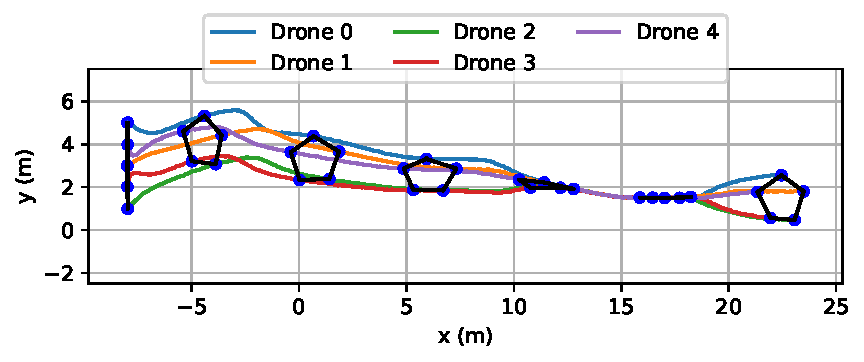
\includegraphics[width=\textwidth]{paper3/images/gazebo_path.pdf}
    \caption{The captured motion paths}
    \label{fig:gazebo_path}
    \end{subfigure}
    \begin{subfigure}[b]{0.48\textwidth}
    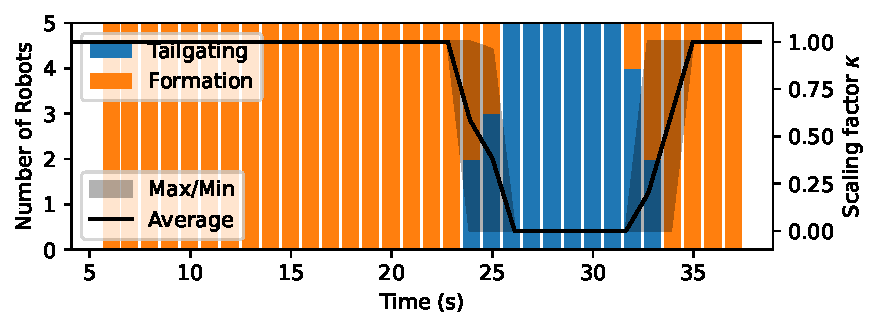
\includegraphics[width=\textwidth]{paper3/images/gazebo_correlation.pdf}
    \caption{Correlation of number of robots and scaling factor $\kappa$}
    \label{fig:gazebo_mode}
    \end{subfigure}
    \begin{subfigure}[b]{0.48\textwidth}
    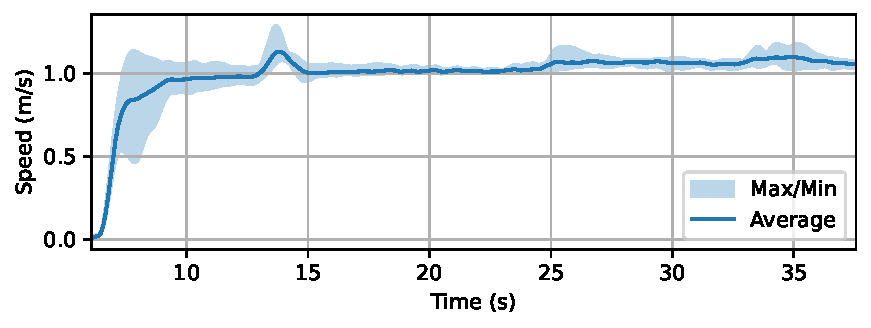
\includegraphics[width=\textwidth]{paper3/images/gazebo_speed.pdf}
    \caption{The speed profile}
    \label{fig:gazebo_speed}
    \end{subfigure}
    \begin{subfigure}[b]{0.48\textwidth}
    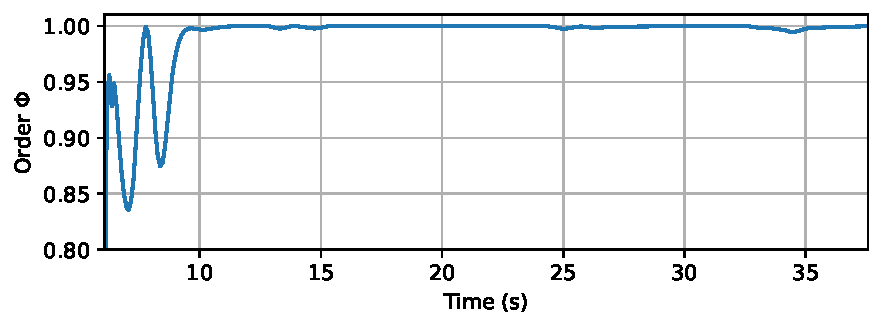
\includegraphics[width=\textwidth]{paper3/images/gazebo_order.pdf}
    \caption{The \textit{order} metric $\Phi$}
    \label{fig:gazebo_order}
    \end{subfigure}
    \begin{subfigure}[b]{0.48\textwidth}
    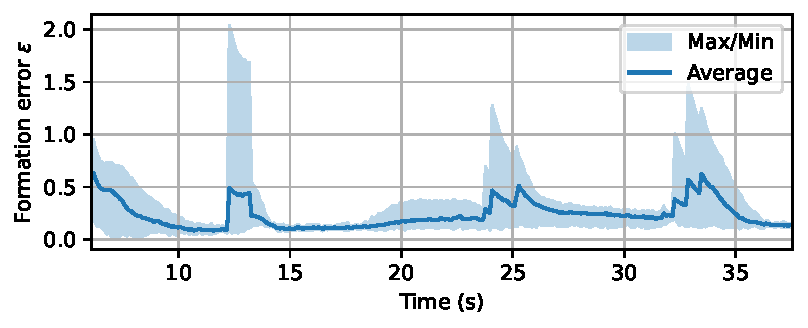
\includegraphics[width=\textwidth]{paper3/images/gazebo_error.pdf}
    \caption{The \textit{formation error} $\varepsilon_i$}
    \label{fig:gazebo_error}
    \end{subfigure}
    \begin{subfigure}[b]{0.48\textwidth}
    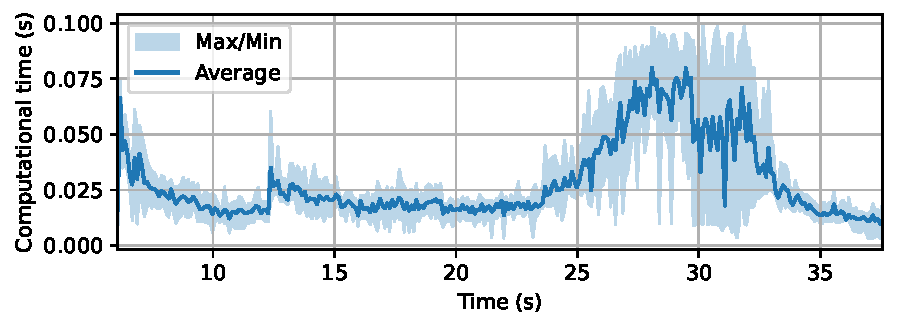
\includegraphics[width=\textwidth]{paper3/images/gazebo_computation.pdf}
    \caption{The computational times}
    \label{fig:gazebo_time}
    \end{subfigure}
    \caption{The recorded results and metrics in the SIL test}
    \label{fig:gazebo}
\end{figure*}

For the further performance assessment of the proposed control strategy, we have carried out software-in-the-loop (SIL) tests, as illustrated in Fig.~\ref{fig:sil}, whose environment is a narrow space that consists of two large obstacles form a cave-like environment with different widths in each area in Gazebo simulator, as shown in Fig.~\ref{fig:gazebo_tunnel}. We set up five homogeneous Hummingbird quadrotors\footnote{Source code used to setup Gazebo SIL test - {\tt\url{https://github.com/duynamrcv/hummingbird_simulator}}} developed based on the RotorS simulator~\cite{Furrer2016} with an arm length of 0.17~m and a mass of 0.716~kg, the rotor thrust constant is $1.6\time10^{-2}$~N/A and the rotor drag constant is $8.54858\times10^{-6}$~Nm/A, as depicted in Fig.~\ref{fig:gazebo_hummingbird}. Each UAV is equipped with local sensors that provide point cloud data of the environment, a positioning module that supplies location information, and a communication module for interacting with other UAVs.

Fig.~\ref{fig:snap} depicts the migration process of a formation passing through the narrow space. It can be seen that a formation can successfully move through the tight passage without collision. During the movement process, a formation can adapt its shape based on the width of passages, which is measured and estimated by each UAV, which can be described in Fig.~\ref{fig:gazebo_path}. Fig.~\ref{fig:gazebo} provides in detail the results of the SIL test. According to Fig.~\ref{fig:gazebo_mode}, each UAV can self-assign its mode based on the perception of the surrounding environment. The formation shrinks as the environment shrinks, described by the $\kappa$ value, as illustrated in Fig.~\ref{fig:gazebo_mode}. Drones in the formation transform to the \textit{``Tailgating''} mode when the narrow space is detected. The requirements for the movement mission on the speed, order, and formation keeping are also guaranteed, as depicted in Fig.~\ref{fig:gazebo_speed}-\ref{fig:gazebo_order}-\ref{fig:gazebo_error}. Moreover, the computational time to handle each iteration of the controller can be reported in Fig.~\ref{fig:gazebo_time}. It can be confirmed that the performance of the proposed control can be successfully deployed for the system.

\subsection{Discussion}
Through the results of simulation experiments, we show the  key properties of the proposed strategy as follows:

\subsubsection{Decentralization} \textit{MPPRFC} is a fully decentralized control. Each robot's decisions are based solely on its own local sensor perceptions. Unlike the approach in~\cite{AlonsoMora2018} which requires network-wide communication under limited communication to update the information of all robots, the \textit{MPPRFC} utilizes only one-hop communication between each robot and its neighbors to update predictive states.

\subsubsection{High performance}

The simulation results in \ref{subsec:results} show that \textit{MPPRFC} successfully navigates robots through narrow environments, ensuring high-performance indicators such as low formation error, stable formation direction, and consistent speed. In contrast to the studies in~\cite{Elkilany2020,Vsrhelyi2018,Soria2021,AlonsoMora2018} which only shrink or expand the formation to adapt to changing space and have no evidence of movement through very narrow spaces, \textit{MPPRFC} enables the robot formation to transition into a tailgating (one-chain) configuration, allowing the robots to easily move through the very narrow spaces one at a time.

\subsubsection{Scalability}
The \textit{MPPRFC} algorithm is successfully implemented with variable-sized robot swarms of 4, 5, 6, 7, 10, 15, and 20 robots without requiring any modifications to the algorithm. The measurement metrics of the swarm indicate that the requirements are satisfied, proving that \textit{MPPRFC} is scalable and maintains efficiency across different swarm sizes. 

\subsubsection{Flexibility}
The \textit{MPPRFC} algorithm provides flexibility and adaptability to different environmental geometries, automatically adjusting structures based on the scaling factor $\kappa$ in Eq.~\eqref{eqn:kappa} obtained from local sensor perceptual information. By analyzing and processing data from local sensors equipped on the robot, the swarm can adapt to numerous environmental structures. In narrow spaces, the proposed algorithm provides each robot with the ability for distributed decision-making, i.e., the formation can shrink/expand or transform to a straight line, to navigate effectively and safely. The \textit{MPPRFC} was also investigated on a simulation platform that replicates the physical environment, demonstrating its potential for applications in real-world scenarios.